\documentclass[10pt,twocolumn]{article}

% ---- Page geometry -----------------------------------------------------
\usepackage[a4paper,margin=1.9cm,columnsep=0.7cm]{geometry}

% ---- Fonts / encoding ----------------------------------------------------
\usepackage[T1]{fontenc}
\usepackage[utf8]{inputenc}
\usepackage{newtxtext,newtxmath}
\usepackage{microtype}

% ---- Math / tables / figures ---------------------------------------------
% amssymb omitted: newtxmath already supplies the AMS symbol fonts, and
% loading both makes them fight over \Bbbk.
\usepackage{amsmath}
\usepackage{graphicx}
\usepackage{booktabs}
\usepackage{caption}
\usepackage{enumitem}

% ---- References -----------------------------------------------------------
\usepackage[numbers,sort&compress]{natbib}

% ---- Section styling (IOP/JNE-like: bold run-in, numbered) ---------------
\usepackage{titlesec}
\titleformat{\section}{\normalfont\large\bfseries}{\thesection.}{0.6em}{}
\titleformat{\subsection}{\normalfont\bfseries}{\thesubsection.}{0.6em}{}
\titlespacing*{\section}{0pt}{1.4ex plus 1ex minus .2ex}{0.8ex plus .2ex}
\titlespacing*{\subsection}{0pt}{1.1ex plus 1ex minus .2ex}{0.6ex plus .2ex}

% ---- Hyperlinks (load last) -----------------------------------------------
\usepackage[colorlinks=true,linkcolor=black,citecolor=black,urlcolor=blue,
            breaklinks=true]{hyperref}

\newcommand{\pptwo}{\texttt{pulse2percept}}
\newcommand{\um}{\ensuremath{\mu\text{m}}}
\newcommand{\uA}{\ensuremath{\mu\text{A}}}

\setlength{\parskip}{0pt}
\setlength{\parindent}{1em}

\title{\bfseries Divisive Normalisation as the Origin of Electrode
Interaction in Cortical Visual Prostheses}

\author{\normalsize Animesh Ratna$^{1}$}
\date{}

\begin{document}
\twocolumn[
  \begin{@twocolumnfalse}
    \maketitle
    \vspace{-1.2em}

    \begin{center}
    \begin{minipage}{0.92\textwidth}
    \small
    \noindent\textbf{Keywords:} visual prosthesis, visual cortex, phosphene,
    divisive normalisation, computational model, neurostimulation

    \bigskip
    \begin{center}\textbf{\normalsize Abstract}\end{center}

    \noindent Simulators of cortical visual prostheses
    represent electrodes as independent, each generating a Gaussian
    phosphene at its retinotopic position, with percepts combining by linear
    superposition. This assumption is load-bearing, as stimulus encoders are
    optimised against these simulators. The present study investigates which
    properties of primary visual cortex, if any, invalidate this assumption,
    and whether the distinction has consequences for device programming.

    \smallskip
    \noindent A forward model was implemented that adds
    two properties omitted from existing simulators --- long-range
    horizontal connections between iso-orientation domains, and divisive
    normalisation --- within the \pptwo{} framework. Every configuration was
    calibrated to reproduce the single-electrode phosphene
    size-versus-current data published for the Dynaphos baseline, so that
    all configurations agree on single-electrode behaviour and differ only
    in their prediction for multi-electrode stimulation. Percepts were
    estimated using a decoder fitted to the model's own normal-vision
    pathway rather than assumed from retinotopy.

    \smallskip
    \noindent Linear mechanisms are shown to be
    incapable of breaking electrode independence: orientation-selective
    horizontal spread produces zero interaction ($<10^{-9}$) at every
    separation and gain tested, a consequence of linearity rather than of
    parameter choice. Divisive normalisation, by contrast, produces
    suppressive interaction of 19--44\% peaking at 1.2--1.6~mm separation and
    decaying to noise by approximately 4.5~mm at 300~\uA. A 32-fold change in
    normalisation strength alters the magnitude roughly two-fold while
    leaving the length scales unchanged, and single-electrode psychophysics
    is found to be incapable of constraining that strength. Against
    published human multi-electrode data at matched stimulation currents,
    the model predicts 38.9\% interaction at the separation where phosphenes
    are reported to merge and 0.0\% where two distinct phosphenes are
    reported, with no parameter adjusted for fit. Stimulation optimised
    against the independent model incurs only a 0.6\% loss of pattern
    fidelity but delivers percepts at 39\% of intended contrast, a shortfall
    that a brightness-sensitive objective improves only to 44\%, at further
    cost to pattern fidelity, and that a scale-invariant objective cannot
    detect.

    \smallskip
    \noindent Electrode interaction in cortex is
    dynamic rather than geometric in origin, and consequently cannot be
    captured by adding anatomical detail to a linear forward model. Its
    principal practical consequence is a brightness shortfall that current
    encoder-evaluation practice does not reveal.
    \end{minipage}
    \end{center}
    \bigskip
  \end{@twocolumnfalse}
]

% \footnotetext used inside \twocolumn[...]'s optional argument is silently
% dropped -- that argument is typeset into a box outside the normal
% page-output flow, so the footnote never reaches the page. Placed here,
% back in ordinary flow, it correctly renders at the bottom of page 1.
\footnotetext[1]{Birla Institute of Technology and Science, Pilani.
  Corresponding author: \texttt{f20240665@pilani.bits-pilani.ac.in}}

\section{Introduction}

A cortical visual prosthesis stimulates primary visual cortex directly,
bypassing the eye and optic nerve. It is the only route to restored vision
when the retina or optic nerve is destroyed --- glaucoma, optic neuropathy,
trauma --- a larger population than retinal implants can serve. Chronic
phosphene generation has been demonstrated safely over 19 months with a
96-channel intracortical array \citep{fernandez2019,nct02983370}, and Phase~I
trials of wireless intracortical devices are underway \citep{nct04634383}.
Recent work predicts phosphene threshold, brightness and number from the
activity of neighbouring electrodes \citep{scienceadv2025}.

Turning stimulation into useful vision is an encoding problem: given a
camera image, which electrodes fire and at what amplitude. The field solves
it by optimising an encoder against a differentiable forward model of what
stimulation produces \citep{granley2022,deruyter2022,rl2022,e2e2025}. For
cortex the state of the art is Dynaphos \citep{vandergrinten2023},
distributed within \pptwo{} \citep{beyeler}. Dynaphos models retinotopy via
a reverse wedge-dipole map, cortical magnification, current spread, and
brightness and threshold as functions of stimulation parameters. It does not
model cortical circuitry, and its documentation states the consequence: each
electrode produces a Gaussian blob, and electrodes are independent.

There is precedent for doubting that. Retinal prosthesis simulation made the
same simplification and it failed: an epiretinal electrode also activates
the ganglion-cell axon bundles passing over it, so percepts are elongated
rather than round and patterns intended as letters become illegible
(figure~\ref{fig:f1}(a),(b)) \citep{beyeler}. The correction was anatomical
--- something the geometric model did not contain.

The assumption is also known to be imperfect empirically. Bosking
\textit{et al.} stimulated 2--6 subdural surface electrodes simultaneously in
11 volunteers and found that concurrent stimulation yields phosphenes
reliably smaller than independent stimulation, and that some pairs produce
one phosphene where two are expected \citep{bosking2022}. They decline to
attribute this to a specific mechanism, raising cortical interaction and
downstream perceptual readout as equally open possibilities. What has been
missing is a mechanism, and a forward model that expresses one.

Existing cortical forward models do not supply it. Dynaphos ships an
optional, non-default multi-electrode extension in which current from active
electrodes leaks to their neighbours in inverse proportion to squared
distance --- a geometric heuristic rather than a circuit mechanism, and one
not evaluated against the separation-dependent interaction magnitudes
Bosking \textit{et al.} report. The most anatomically detailed cortical
virtual patient to date, which also derives receptive fields from a
simulated orientation map, states explicitly that it excludes ``electric
field or nonlinear neural interactions'' between electrodes and assumes
percepts sum linearly throughout \citep{fineboynton2024}; its orientation
map shapes the elongation of single-electrode receptive fields and does not
mediate any spread of activation between electrodes. Neither model tests
electrode independence, and neither is compared against multi-electrode
interaction data.

The obvious cortical analogue of the retinal effect is the long-range
horizontal connection system: superficial pyramidal axons running for
millimetres parallel to the surface and terminating in clusters on columns
of similar orientation preference \citep{gilbert1983,kandel2013}. We set out
to test whether these produce the cortical equivalent. They cannot, for a
reason that turns out to be more informative than the hypothesis.

\section{Methods}

\subsection{Baseline and verification of the independence assumption}

All comparisons use \pptwo{} 0.9.1 with the \texttt{Cortivis} implant
geometry and \texttt{Polimeni2006Map} retinotopy. The baseline is
\texttt{cortex.DynaphosModel} with default parameters, driven by 300~Hz
biphasic pulse trains (170~\um{}s per phase, 100~ms burst).

We verified independence empirically rather than assuming it from
documentation. For two electrodes 0.8\textdegree{} apart in the visual field
at 200~\uA, the maximum relative deviation from linear superposition was
$3.7\times10^{-9}$ (figure~\ref{fig:f1}(c),(d)) --- floating-point noise.
Superposition holds exactly.

\subsection{Circuit model}

\texttt{CircuitSpatial} is implemented as a \pptwo{} spatial model so that
the comparison is like-for-like. Activation is computed on a uniform
cortical sheet (50~\um{} resolution) and read out at each visual-field grid
point through the same retinotopy the implant uses.

\textit{Current spread} reproduces Dynaphos: activated tissue diameter
$D = 2\sqrt{I/K}$. Activation magnitude additionally scales with a
saturating function of amplitude, which leaves the half-maximum contour, and
therefore the size calibration, unchanged.

\textit{Orientation map.} Iso-orientation domains are generated by
band-pass filtering complex Gaussian noise and halving its phase
\citep{rojer1990}, giving quasi-periodic domains joined at pinwheels with a
macaque V1 column spacing of $\sim$750~\um{} (figure~\ref{fig:f2}(a)).

\textit{Horizontal connections.} Activation spreads to sites weighted by
cortical distance ($\sigma = 1$~mm) and orientation similarity
($\sigma = 27$\textdegree). Expanding the orientation term to first Fourier
order reduces this to three Gaussian convolutions,
\begin{equation}
  \frac{G(A) + r\cos2\theta\, G(A\cos2\theta) + r\sin2\theta\, G(A\sin2\theta)}
       {1+r},
\end{equation}
which keeps a millimetre-scale sheet tractable and the model
differentiable.

\textit{Divisive normalisation} \citep{carandini2012}: each site's expansive
response is divided by a Gaussian-pooled measure of neighbourhood activity
($\sigma = 1.5$~mm). An optional second, broader pool is described in
section~\ref{sec:s35}.

Both mechanisms can be disabled independently; with both off the model
reduces to pure current spread, the control condition that makes any
difference attributable to the circuit rather than to a different spread
model.

\subsection{Calibration}

Every configuration was fitted, by adjusting $K$ alone, to reproduce the
baseline's single-electrode phosphene diameter across 100--600~\uA{}
(figure~\ref{fig:f2}(b)). Mean absolute error was 2.3\% (circuit off), 2.4\%
(horizontal only), 3.7\% (normalisation only) and 4.0\% (both). All
configurations therefore agree with the published single-electrode data and
with each other.

\subsection{Percept decoder}

To make claims about percepts rather than activation we fitted a readout.
Each cortical site is an oriented filter with a receptive-field position
from the retinotopy, an orientation from the map, and a spatial phase. The
predicted percept is the image that best explains the observed activity,
\begin{equation}
  \operatorname*{minimise}_{I}\ \lVert MI - a\rVert^2 + \lambda\lVert\nabla I\rVert^2,
\end{equation}
solved on the same forward operator used for encoding. We use this rather
than regressing images on activity: a ridge decoder achieves comparable
reconstruction on natural images ($R^2$ 0.65 against 0.66) but produces
structured speckle on stimulation, because it estimates
$\mathbb{E}[\text{image}\mid\text{activity}]$ under a training distribution
that stimulation is nowhere near --- visual input drives a site only if the
stimulus matches its tuning, whereas an electrode drives every nearby site
regardless.

Held-out reconstruction $R^2 = 0.66$ on $1/f$ noise images
(figure~\ref{fig:f6}(a)). Reconstruction resolution optimises at
$\sim$0.15\textdegree/pixel and degrades either side. This is the
hypercolumn limit: a full set of orientations and phases occupies
$\sim$750~\um{} $\approx$ 0.18\textdegree{} of visual field at this
eccentricity, and sampling cortex more finely does not help because
neighbouring sites carry different orientations rather than repeating a
measurement.

\subsection{Optimal stimulation}

For encoder consequences we avoided training a network, which would
confound forward-model accuracy with network capacity. For each target we
solved directly for the amplitude vector maximising percept fidelity under a
given forward model (L-BFGS-B, 24 electrodes, 0--600~\uA), which is the best
any encoder of any architecture could achieve given that model.

Targets were defined as percepts the device can actually deliver. An
initial attempt using geometric shapes produced fidelities of 0.001--0.06;
fitting those targets with an unconstrained linear combination of
single-electrode percepts reached only 0.03--0.15, establishing that a
couple of dozen phosphenes cannot render a thin bar in a 256-pixel image at
any amplitude. Asking what a modelling error costs is meaningless when there
is no fidelity to lose.

Pattern fidelity is reported as squared correlation and percept brightness
as RMS contrast relative to target, with both models anchored to identical
single-electrode brightness so that the comparison is not an artefact of
differing activation scales.

\section{Results}

\subsection{Linear mechanisms cannot break independence}

Orientation-selective horizontal spread produces no departure from
superposition: below $10^{-9}$ at every separation (400--2400~\um) and gain
(0.3--1.2) tested (figure~\ref{fig:f3}(a), dashed line at zero).

The reason is structural rather than numerical. Horizontal spread as
implemented --- and in any convolutional formulation --- is a linear
operator, and $L(A+B) = L(A) + L(B)$ by definition. No connectivity rule,
however orientation-selective or anatomically detailed, can create electrode
interaction if it acts linearly.

This was contrary to our expectation and disanalogises the cortical case
from the retinal one. The axon-bundle effect is \textit{geometric}: it
changes the shape of a single phosphene, and a linear model captures it,
which is why the axon-map model works. A cortical interaction effect must be
\textit{dynamic}, and no linear extension of any current baseline can
express it.

\subsection{Divisive normalisation does break it}

With normalisation enabled, departure from superposition at 300~\uA{} per
electrode reaches 24.7\% and is suppressive --- a pair produces less than
the sum (figure~\ref{fig:f3}(a), table~\ref{tab:t1}). It peaks near the
pooling scale and is negligible beyond $\sim$4.5~mm. Cortivis electrode
pitch is 400~\um{} and the array spans $\sim$4~mm, so the affected range is
the range real arrays occupy. Perceptually, two electrodes 1.44~mm apart
that the baseline renders as two distinct spots merge into a single
elongated percept (figure~\ref{fig:f3}(b)--(d)).

\begin{table}[t]
\centering
\caption{Departure from linear superposition (\%), 300~\uA{} per electrode.}
\label{tab:t1}
\small
\setlength{\tabcolsep}{3.2pt}
\begin{tabular}{lccccccc}
\toprule
sep. (mm) & 0.4 & 0.8 & 1.2 & 1.6 & 2.4 & 3.2 & 4.5 \\
\midrule
Dynaphos baseline    & 0 & 0 & 0 & 0 & 0 & 0 & 0 \\
circuit off          & 0 & 0 & 0 & 0 & 0 & 0 & 0 \\
horizontal only      & 0 & 0 & 0 & 0 & 0 & 0 & 0 \\
normalisation only   & 11.8 & 10.8 & 18.9 & 22.4 & 15.6 & 7.1 & 1.2 \\
full circuit         & 18.0 & 14.9 & 22.1 & \textbf{24.7} & 17.0 & 8.0 & 1.4 \\
\bottomrule
\end{tabular}
\end{table}

\subsection{The conclusion survives not knowing the parameters}

Normalisation strength is not calibrated by any public data. Sweeping it
over 32-fold (0.25--8) and refitting $K$ at every point so that all models
still reproduce the single-electrode curve, the peak deviation spans
19--44\% while the local-peak separation stays at 1.2--1.6~mm and the
half-decay distance at 2.2--2.8~mm (figure~\ref{fig:f4}(a),(b)). Sweeping
the pooling extent instead walks the peak from 400~\um{} to 2000~\um{}
(figure~\ref{fig:f4}(c)), confirming that geometry is set by the pool and
magnitude by the gain, separably.

The smallest gain is an outlier on both counts and we report it rather than
smooth it: refitting $K$ at each sweep point means gain and operating point
are not fully independent. The monotonic trend from 0.5 to 8 is the
interpretable part.

Every strength from 0.25 to 8 fits the single-electrode curve to within
3--4\%. \textbf{Single-electrode psychophysics therefore cannot constrain
normalisation strength}, and multi-electrode measurement is the only route
to it.

\subsection{Comparison with human multi-electrode data}

The model was built without reference to multi-electrode measurements, so
comparison with them is a test rather than a fit.

Bosking \textit{et al.} \citep{bosking2022} stimulated 2--6 subdural surface
electrodes simultaneously in 11 volunteers, analysing 232 pairs. For pairs
perceived as two distinct phosphenes, sizes under concurrent stimulation
were consistently smaller than under independent stimulation
(2.49\textdegree{} against 3.59\textdegree, $t(34)=8.14$, $p<0.001$,
$n=35$); a second class produced one phosphene where two were expected.
Both are suppressive interactions, in the direction divisive normalisation
predicts and in a direction no independent model can produce.

Comparing spatial scale requires matching stimulation regime. Those
experiments delivered 0.3--4.0~mA; our intracortical predictions were
computed at 300~\uA, and under the model's own current-spread law the
activated radius grows as $\sqrt{I}$, from 0.70~mm to 2.57~mm across that
range. Sweeping amplitude and changing nothing else (figure~\ref{fig:f5},
table~\ref{tab:t2}), at the top of their range the model predicts strong
interaction where percepts merge and overlap both individual phosphenes
(38.9\% at 4.11~mm) and none where two distinct phosphenes are reported
(0.0\% at 26.36~mm). It separates the regimes correctly with no parameter
adjusted to make it do so.

\begin{table}[t]
\centering
\caption{Model interaction (\%) at the mean separations reported in
  \citep{bosking2022}, as a function of stimulation amplitude.}
\label{tab:t2}
\small
\setlength{\tabcolsep}{3.2pt}
\begin{tabular}{lcccc}
\toprule
stimulation & 4.11~mm & 9.57~mm & 26.36~mm & decay \\
            & (merged) &        & (two ph.) & to 10\% \\
\midrule
0.3~mA & 2.5  & 0.0 & 0.0 & 4.4~mm \\
1.0~mA & 12.0 & 0.0 & 0.0 & 5.2~mm \\
2.0~mA & 22.5 & 1.0 & 0.0 & 6.4~mm \\
4.0~mA & \textbf{38.9} & 3.2 & \textbf{0.0} & 8.8~mm \\
\bottomrule
\end{tabular}
\end{table}

That study measured phosphene number, size, location and eccentricity, but
not brightness, so our central percept prediction (section~\ref{sec:s38})
is neither supported nor contradicted by it.

\subsection{Long-range single-phosphene suppression is not normalisation}
\label{sec:s35}

One class of pairs in \citep{bosking2022}, at a mean separation of
13.47~mm ($n=9$), yields one phosphene with the other unreported. The model
predicts under 2\% interaction there.

V1 surround suppression comprises a near component with the reach of
horizontal connections and a far component mediated by extrastriate
feedback with much larger receptive fields. We added the second as an
independent pool and asked whether it can produce suppression at 13.5~mm
while preserving the regimes of section~3.4. It can, but only at one tested
setting: a pool of $\sigma = 8$~mm with \textbf{thirty times} the gain of
the near pool (40.3\%, 16.6\%, 0.6\% at 4.11, 13.47 and 26.36~mm). Every
physiologically ordered setting, in which far suppression is weaker than
near, produces at most 2--6\% at 13.5~mm.

The arithmetic is straightforward: two electrodes 13.5~mm apart contribute
$\exp(-13.5^2/2\sigma^2)\approx0.24$ of peak to each other's pool at
$\sigma=8$~mm, so for that to change the response by more than 15\% the
pooled term must dominate the semi-saturation constant, which requires
large gain. We make no stronger structural claim, since the dependence of
interaction on pool width is not monotonic and at short separations a
broader pool increases rather than decreases the departure from
superposition.

We do not fit this. The original authors do not claim the effect is
cortical: they raise non-uniform spatial attention as a candidate and state
that resolving it will require direct measurement of activity in early
visual areas \citep{bosking2022}. A forward model of cortical activation
should not be expected to reproduce a percept that may be selected after
cortex. Section~\ref{sec:experiments} proposes an experiment that decides
the question.

\subsection{Interaction range scales with stimulation current}

Holding all parameters fixed and varying only amplitude, the distance at
which interaction has decayed to a tenth of its peak grows from 4.4~mm at
0.3~mA to 8.8~mm at 4.0~mA (figure~\ref{fig:f5}, table~\ref{tab:t2}). The
mechanism is transparent: activated radius goes as $\sqrt{I}$, and two
electrodes interact when their activation overlaps the same normalisation
pool.

The spatial extent of electrode interaction is therefore not a fixed
property of cortex but a function of how hard the device is driven.
Interaction measured at threshold currents will understate interaction at
the suprathreshold currents a device uses.

\subsection{Percept-level consequences}

Decoding five simultaneously driven electrodes, activation changes by
32.1\% relative to the independent prediction and the decoded percept by
31.2\% (figure~\ref{fig:f6}(b)). The interaction is neither washed out by
the readout nor amplified; it transfers approximately one-for-one, taking
the form of a fairly uniform suppression of the whole percept rather than a
distortion of its shape.

\subsection{Encoder consequences: the pattern survives, the brightness does not}
\label{sec:s38}

Optimal stimulation computed under each forward model and cross-evaluated
(figure~\ref{fig:f7}) gives a mean pattern fidelity of 0.995 when programmed
for the circuit and delivered to it, against 0.990 when programmed as
independent and delivered to the circuit --- 0.6\% forgone. On this axis the
result is a null: the circuit's suppression is a smooth, largely invertible
distortion that a re-optimised encoder undoes.

On brightness it is not. The delivered percept carries 39\% of the intended
contrast. An objective that actively seeks brightness recovers it only to
44\% and sacrifices pattern fidelity (0.995 $\to$ 0.949) to do so. The
amplitude bound is never reached, so this is not a current limit; it is
what divisive normalisation is. Driving harder recruits more of the pool
that divides, so the suppression cannot be out-driven.

\subsection{Neither metric rescues the brightness}

Both conclusions come from the same percepts and differ only in scoring.
Squared correlation is invariant to scale: a percept of correct shape at
39\% brightness scores identically to one at full brightness. An evaluation
using it alone would report near-perfect success while delivering under
half the intended contrast.

This is a caution about evaluation practice rather than a criticism of
published encoders, several of which optimise scale-sensitive
reconstruction losses \citep{granley2022,deruyter2022}. But a
scale-sensitive objective does not solve the problem, it only reveals it, as
the 0.39 $\to$ 0.44 recovery shows. The shortfall is a property of the
circuit, not of the metric; the metric determines only whether one notices.

\section{Discussion}

\subsection{Proposed experiments}
\label{sec:experiments}

\textbf{Interaction range should scale with current.} The distance over
which electrodes interact is predicted to grow as $\sqrt{I}$, from
$\sim$4.4~mm at 0.3~mA to $\sim$8.8~mm at 4.0~mA. Repeating a
paired-stimulation protocol at two well-separated amplitudes should move
the separation at which merging gives way to two distinct phosphenes.
Independent models predict no interaction at any current, and a
fixed-radius interaction model predicts no shift with amplitude, so the
three are cleanly distinguishable.

\textbf{Shape of the function at intracortical pitches.} At 300~\uA{} the
model predicts interaction is not monotonic in separation, with an interior
maximum near 1.2--1.6~mm and weaker effects at both 0.4~mm and 3~mm.
Measuring phosphene size or brightness at three or four separations
spanning 0.4--3~mm would test this. Because the length scales are
parameter-independent while the magnitude is not, the shape tests the model
and the magnitude estimates normalisation strength --- the separation of
peak suppression measuring the cortical normalisation pool extent, a
quantity not otherwise accessible in humans.

\textbf{Is the lost phosphene lost in cortex or after it?} For pairs where
one of two phosphenes goes unreported, measure trial-to-trial consistency.
Consistent loss of the same phosphene implicates a cortical mechanism,
which section~\ref{sec:s35} shows is not divisive normalisation.
Alternation implicates perceptual competition and places the effect outside
a forward model of cortical activation. This is the cheapest of the three
experiments.

\textbf{Ensemble brightness.} Drive $N$ electrodes each individually
producing brightness $B$. Reported ensemble brightness should fall
increasingly below $NB$ as $N$ grows, and increasing current should fail to
close the gap. Independent models predict brightness adds and have no
mechanism for a ceiling current cannot overcome.

\subsection{Implications for device programming}

If the cortex normalises, encoders built on independent forward models get
the pattern approximately right and the brightness substantially wrong, and
no choice of objective recovers it. Three practical consequences follow:
treat ensemble-brightness budgets derived from independent forward models as
optimistic; report a scale-sensitive metric alongside any correlation-based
one so that a shortfall is visible; and do not expect increased current to
close it, because the mechanism that suppresses also scales with drive.

The corollary for modelling is sharper. Because no linear mechanism can
produce electrode interaction (section~3.1), a forward model intended to
capture it must include an explicit nonlinearity. Adding anatomical detail
to a linear model --- finer retinotopy, richer connectivity,
patient-specific maps --- cannot help, however accurate that detail is.

\subsection{Limitations}

\begin{itemize}[leftmargin=1.1em,itemsep=0.2em,topsep=0.2em]
\item \textbf{Normalisation strength is unconstrained.} Section~3.3 shows
  existing single-electrode data cannot pin it. The 24.7\% and 39\% figures
  are contingent; the direction, mechanism and length scales are not.
\item \textbf{Long-range single-phosphene suppression is deliberately not
  modelled} (section~\ref{sec:s35}). If that effect proves consistent
  trial-to-trial, the model owes an explanation.
\item \textbf{The percept decoder has never been compared to a human
  percept.} It is trained on the model's own normal-vision pathway and
  inherits that pathway's inaccuracies. It answers what image is most
  consistent with a given cortical activity pattern according to this model
  of V1.
\item \textbf{A field model, not a spiking one}, chosen to keep the
  comparison with Dynaphos like-for-like and the parameter sweeps
  tractable. Adaptation, spike timing and temporal dynamics beyond the
  baseline's are absent.
\item \textbf{Different electrode regime from the available human data},
  which uses subdural surface contacts (0.5~mm diameter, 2--6~mm spacing)
  delivering current through CSF and dura, against intracortical arrays at
  400~\um{} pitch here.
\item \textbf{One eccentricity, one array geometry, one hemisphere}
  ($\sim$1.8\textdegree{} eccentricity, \texttt{Cortivis}).
\item \textbf{Deafferented cortex is not modelled.} A blind volunteer's V1
  has had no input for years and is homeostatically altered; parameters
  here are from healthy cortex.
\end{itemize}

\section{Conclusion}

Electrode independence is assumed by every current cortical prosthesis
simulator and is exactly true in them by construction. Human data already
shows it is false: concurrently stimulated electrodes produce measurably
smaller phosphenes than independent ones. We find that no linear mechanism
can account for this, including the horizontal connectivity that seemed the
natural cortical analogue of the retinal axon-bundle effect, and that
divisive normalisation can --- reproducing both the direction of the
observed suppression and, once stimulation currents are matched, the
separations at which percepts merge and at which they remain distinct, with
no parameter adjusted to fit. Suppression at intermediate separations
remains unaccounted for and may not be cortical in origin.

The consequence for device programming is not a loss of pattern fidelity,
which re-optimisation recovers, but a brightness shortfall that no
objective recovers, because the drive intended to overcome a divisive
nonlinearity also feeds it.

\section*{Data availability}

All code, the test suite, and scripts regenerating every figure and number
in this manuscript are available in the accompanying repository.
\texttt{prosthesis/run\_all.py} regenerates all results;
\texttt{paper/make\_figures.py} regenerates all figures;
\texttt{paper/verify\_claims.py} asserts every quantitative claim above
against the regenerated output.

\bibliographystyle{unsrtnat}
\bibliography{manuscript}

\clearpage
\onecolumn

\section*{Figures}

\begin{figure}[h!]
\centering
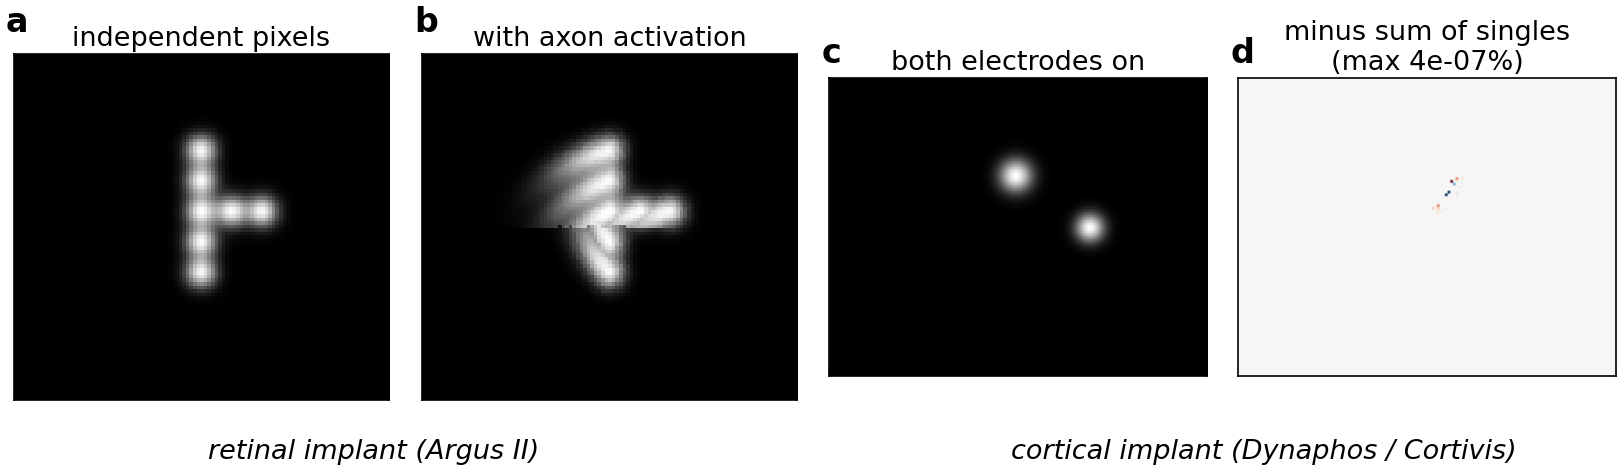
\includegraphics[width=\textwidth]{figures/fig1.png}
\caption{\textbf{The independence assumption and the precedent for doubting
it.} (a) A seven-electrode pattern on an Argus~II retinal implant rendered
by a scoreboard model, in which each electrode is an independent round
phosphene. (b) The same electrodes under an axon-map model that includes
activation of passing ganglion-cell axon bundles; the pattern is no longer
legible. (c) Two Cortivis electrodes driven together at 200~\uA{} under the
Dynaphos cortical baseline. (d) The difference between (c) and the sum of
the two electrodes driven separately: $3.7\times10^{-9}$ of the peak, i.e.
floating-point noise. Superposition holds exactly in the cortical baseline
by construction.}
\label{fig:f1}
\end{figure}

\begin{figure}[h!]
\centering
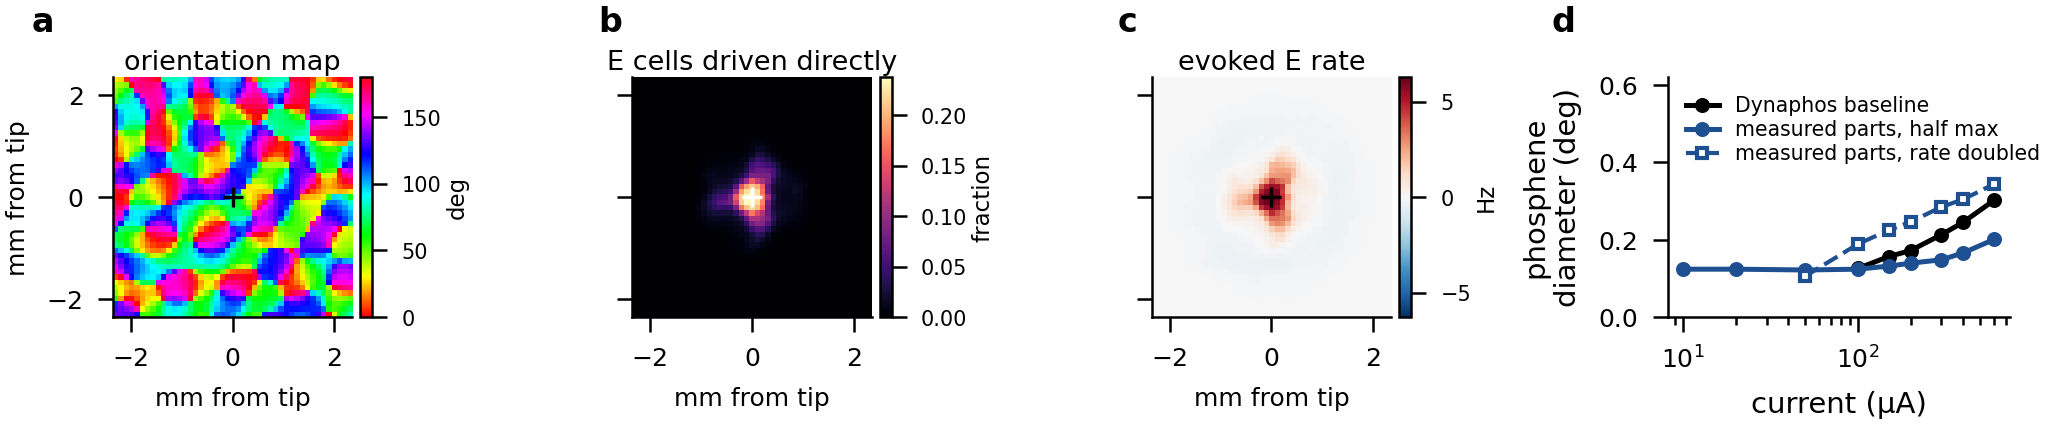
\includegraphics[width=\textwidth]{figures/fig2.png}
\caption{\textbf{Model and calibration.} (a) Simulated V1 orientation
preference map, generated by band-pass filtering complex Gaussian noise,
with a column spacing of 750~\um. (b) Phosphene diameter against stimulus
amplitude for the Dynaphos baseline (black) and for all four configurations
of the circuit model after fitting the excitability constant alone. Legend
gives mean absolute error against the baseline. Every configuration
reproduces the same single-electrode data, so subsequent differences
between them concern only multi-electrode stimulation.}
\label{fig:f2}
\end{figure}

\begin{figure}[h!]
\centering
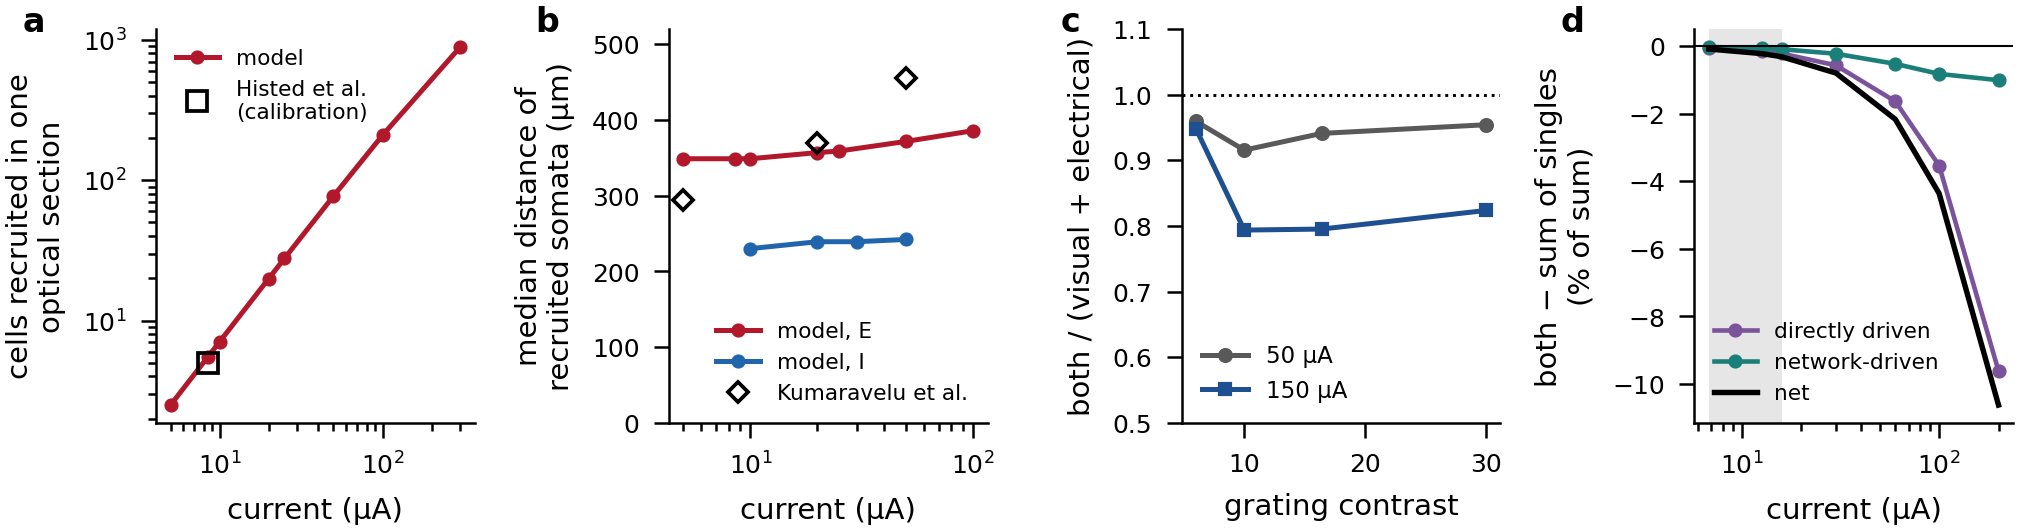
\includegraphics[width=\textwidth]{figures/fig3.png}
\caption{\textbf{Only a nonlinearity breaks electrode independence.} (a)
Departure from linear superposition against electrode separation, 300~\uA{}
per electrode. The circuit-off and horizontal-only curves lie on zero and
on each other; the latter is dashed to remain visible. Orientation-selective
horizontal spread contributes nothing because it is linear. (b)--(d)
Cortical activation for two electrodes 1.44~mm apart: the prediction if the
electrodes were independent (b), the circuit model's prediction (c), and
their difference (d). Two distinct maxima merge into a single elongated
region.}
\label{fig:f3}
\end{figure}

\begin{figure}[h!]
\centering
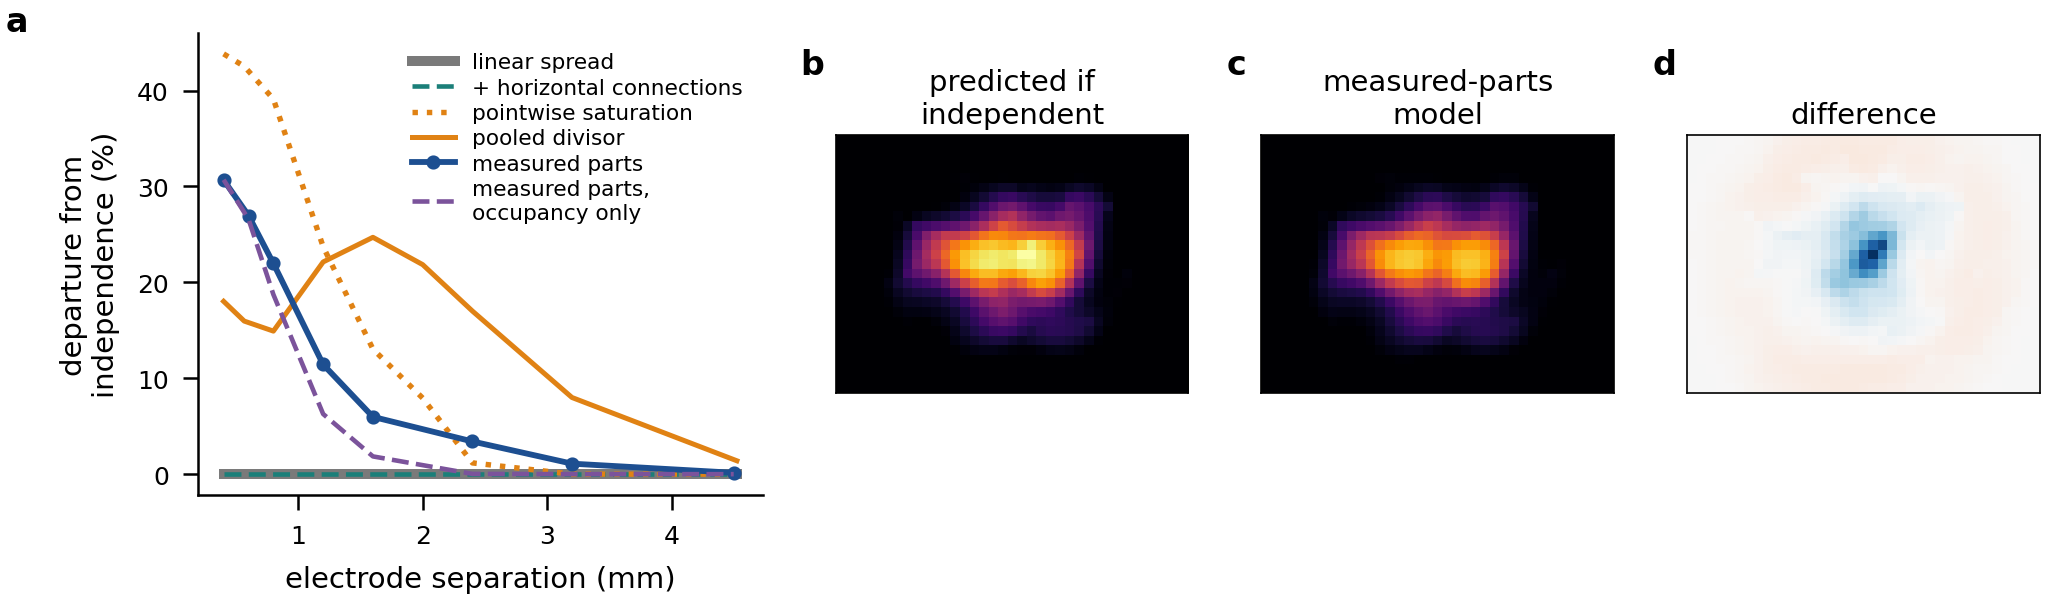
\includegraphics[width=\textwidth]{figures/fig4.png}
\caption{\textbf{Robustness to the uncalibrated normalisation parameters.}
(a) Interaction against separation for normalisation pool gains spanning
32-fold, with the excitability constant refitted at every point so that all
models still reproduce the single-electrode curve. (b) Peak deviation (left
axis) and the separation at which the interior peak occurs (right axis)
against pool gain. Magnitude varies roughly two-fold; the length scale does
not move. (c) The same sweep over pool width instead, which walks the peak
from 0.4~mm to 2~mm.}
\label{fig:f4}
\end{figure}

\begin{figure}[h!]
\centering
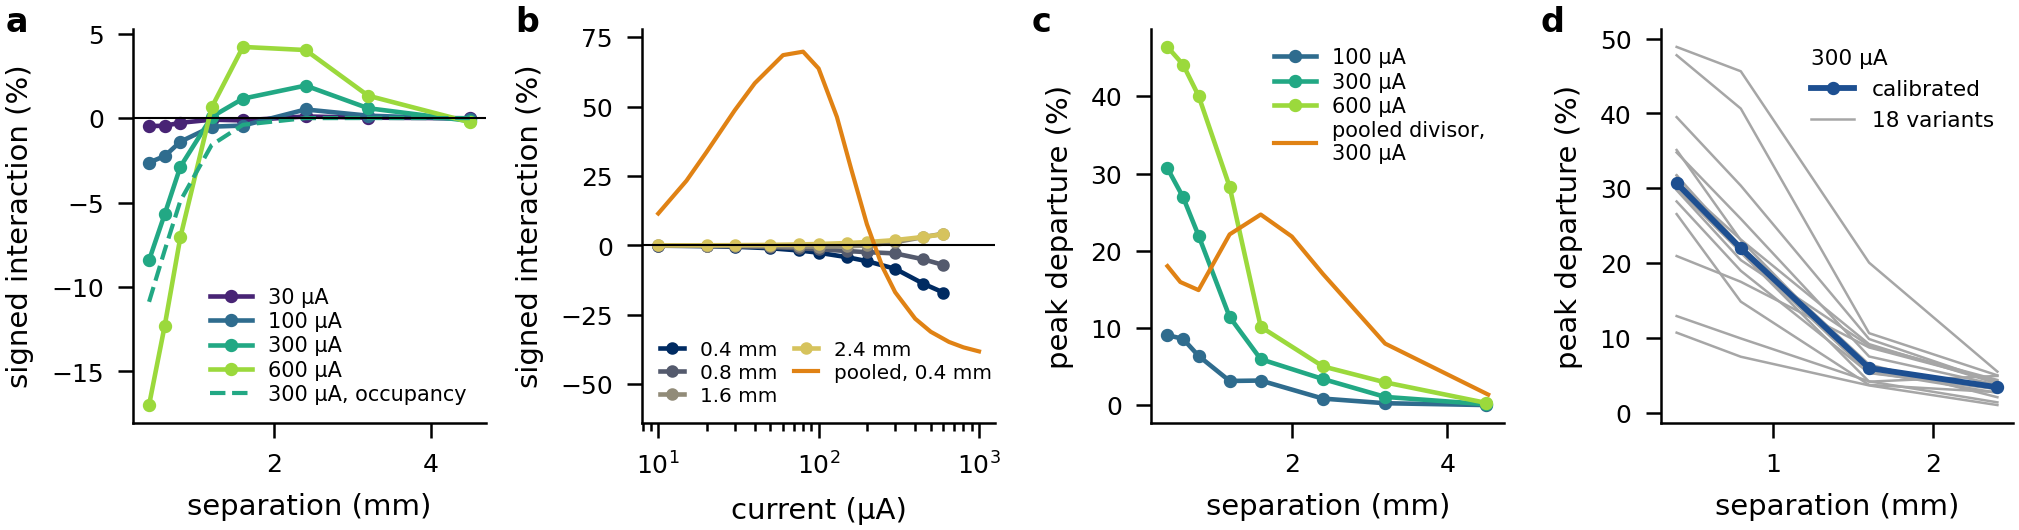
\includegraphics[width=0.7\textwidth]{figures/fig5.png}
\caption{\textbf{Interaction range scales with stimulation current.}
Departure from independence against separation at four amplitudes spanning
the range used in human surface-stimulation experiments, with all other
parameters fixed. Dotted lines mark the mean separations reported in
\citep{bosking2022} for pairs whose phosphenes merged and for pairs
perceived as two distinct phosphenes. At 4~mA the model predicts strong
interaction at the former and none at the latter.}
\label{fig:f5}
\end{figure}

\begin{figure}[h!]
\centering
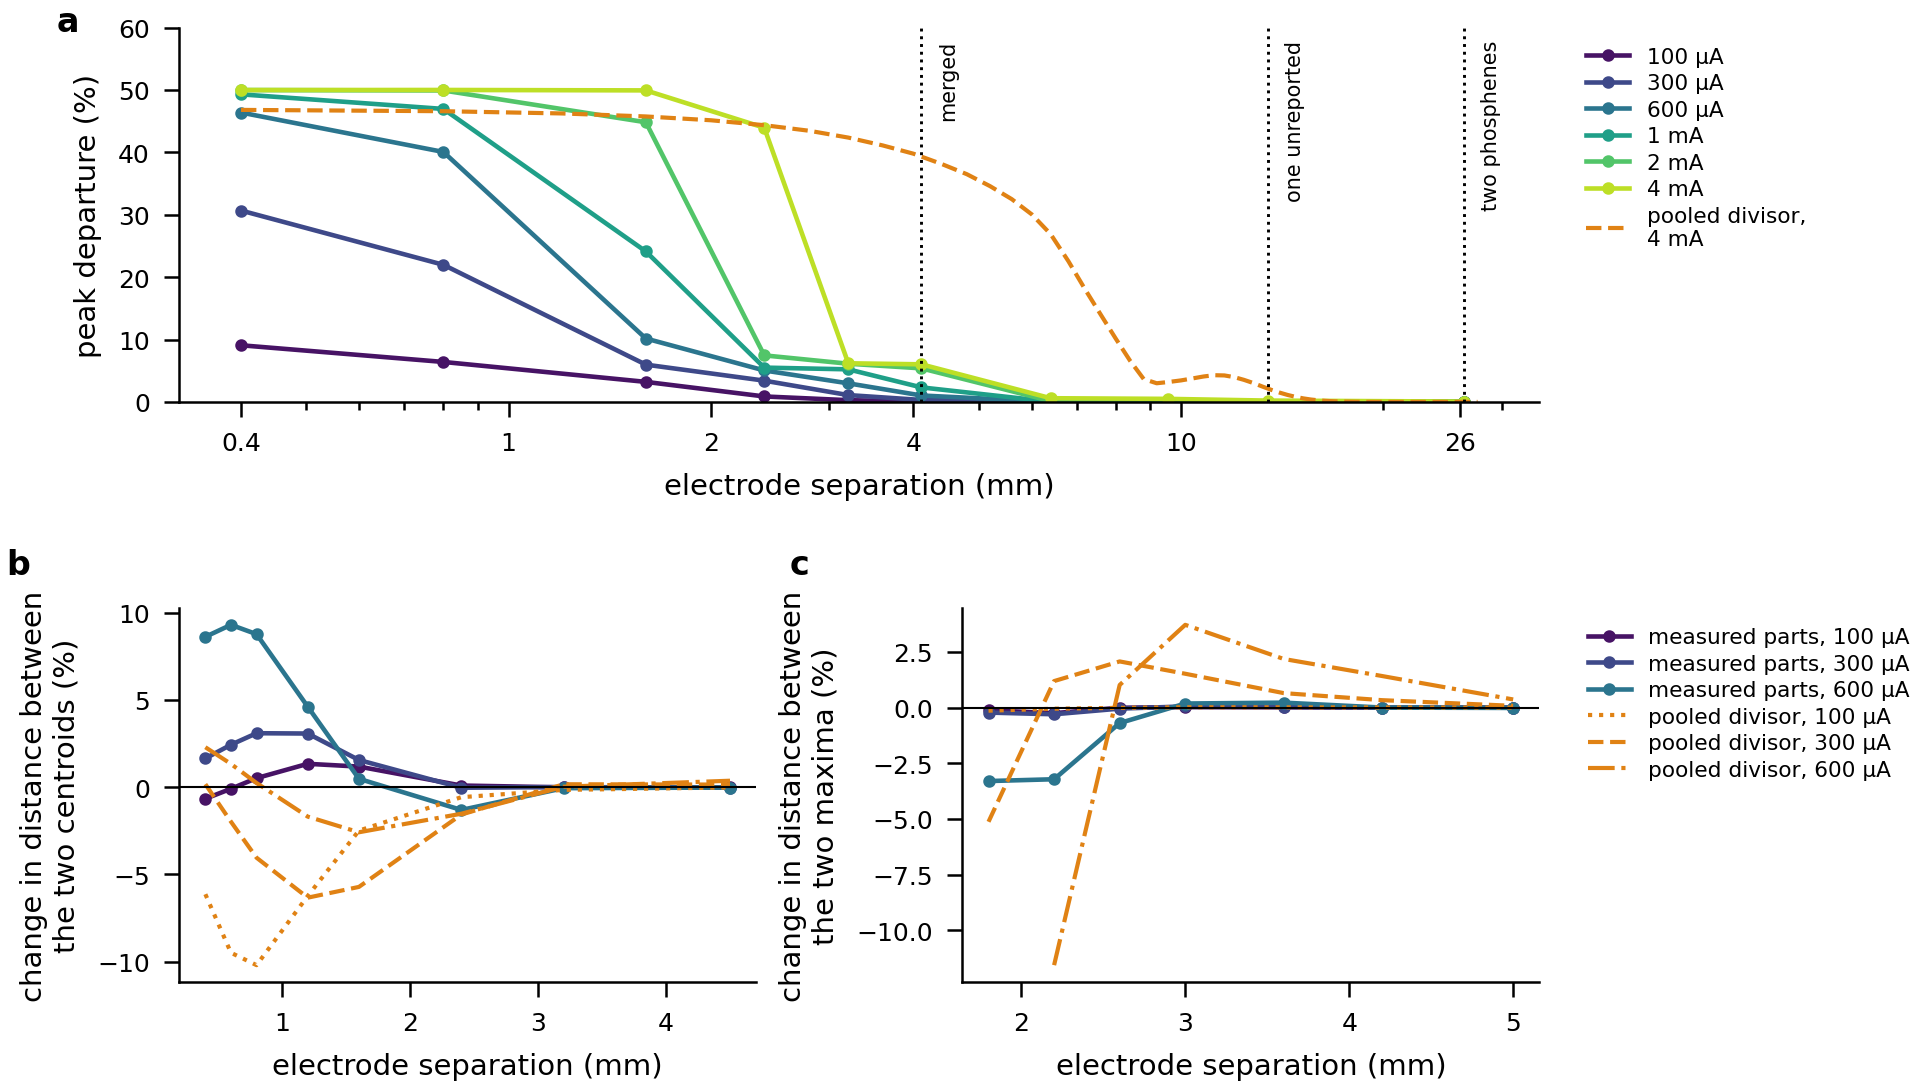
\includegraphics[width=\textwidth]{figures/fig6.png}
\caption{\textbf{Percept prediction.} (a) Held-out validation of the
decoder: $1/f$ noise images shown to the model's normal-vision pathway (top)
and recovered from the resulting cortical activity (bottom); $R^2 = 0.66$,
estimated over 24 held-out images of which four are shown. (b) Predicted
percepts for five electrodes, comparing the sum of the electrodes driven
individually with all five driven together, under the independent
configuration (top) and the circuit (bottom). The circuit suppresses the
percept approximately uniformly.}
\label{fig:f6}
\end{figure}

\begin{figure}[h!]
\centering
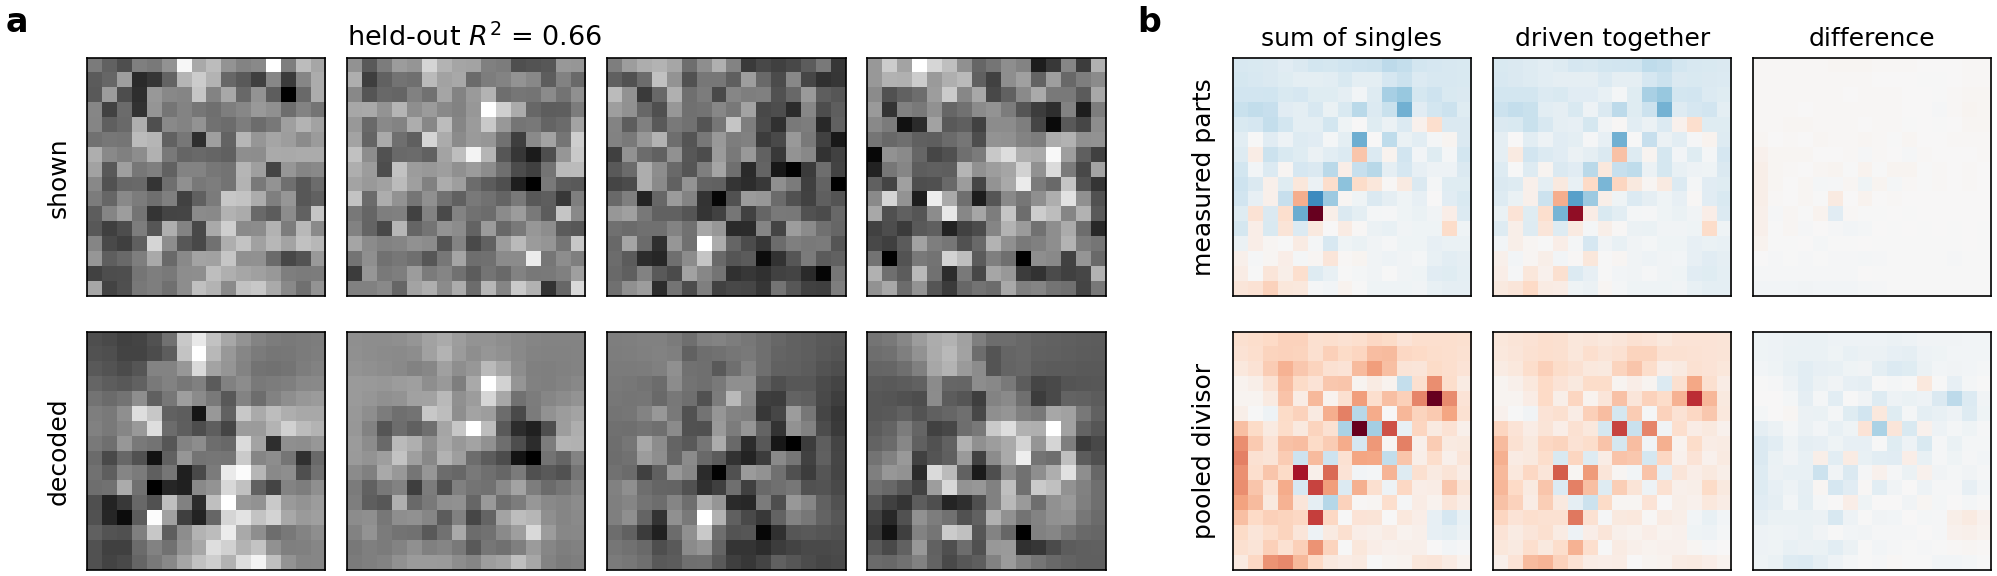
\includegraphics[width=\textwidth]{figures/fig7.png}
\caption{\textbf{Encoder consequences.} (a) Pattern fidelity for six
deliverable target percepts, comparing stimulation optimised for the
circuit and delivered to it against stimulation optimised as though
electrodes were independent and delivered to the circuit. The difference is
0.6\%. (b) Percept contrast relative to target: as delivered, and after
re-optimising an objective that explicitly seeks brightness. The shortfall
is largely irrecoverable.}
\label{fig:f7}
\end{figure}

\end{document}
